\documentclass[tikz,border=8pt]{standalone}
\usepackage{fontspec}
\usepackage{amssymb}
\usepackage{xcolor}
\usetikzlibrary{arrows.meta,calc,positioning,shadows.blur}

\setmainfont{Latin Modern Sans}

\definecolor{substrate}{HTML}{1F4E79}
\definecolor{matter}{HTML}{2E7D32}
\definecolor{gauge}{HTML}{00838F}
\definecolor{cosmo}{HTML}{EF6C00}
\definecolor{dark}{HTML}{6A1B9A}
\definecolor{gravity}{HTML}{B71C1C}
\definecolor{method}{HTML}{616161}
\definecolor{derivedfill}{HTML}{E8F2FF}
\definecolor{condfill}{HTML}{FFF3D6}
\definecolor{openfill}{HTML}{F2E7FA}
\definecolor{importfill}{HTML}{EEEEEE}

\tikzset{
  route/.style={line width=4.2pt, line cap=round, line join=round},
  thinroute/.style={line width=2.0pt, line cap=round, line join=round},
  transfer/.style={
    rounded corners=4pt,
    draw=black!55,
    line width=0.55pt,
    fill=white,
    blur shadow={shadow blur steps=5, shadow xshift=0.5pt, shadow yshift=-0.5pt, shadow opacity=18},
    align=center,
    font=\scriptsize,
    inner xsep=4pt,
    inner ysep=3pt,
    text width=2.35cm
  },
  station/.style={
    rounded corners=3pt,
    draw=black!45,
    line width=0.45pt,
    fill=white,
    align=center,
    font=\scriptsize,
    inner xsep=3pt,
    inner ysep=2.5pt,
    text width=2.15cm
  },
  derived/.style={fill=derivedfill, draw=substrate!65},
  conditional/.style={fill=condfill, draw=cosmo!85},
  open/.style={fill=openfill, draw=dark!80, dashed},
  imported/.style={fill=importfill, draw=method!70},
  proof/.style={font=\tiny\ttfamily, text=black!70, align=center},
  labelbox/.style={font=\scriptsize\bfseries, text=black!78, align=left},
  legend/.style={font=\tiny, align=left, text=black!78}
}

\begin{document}
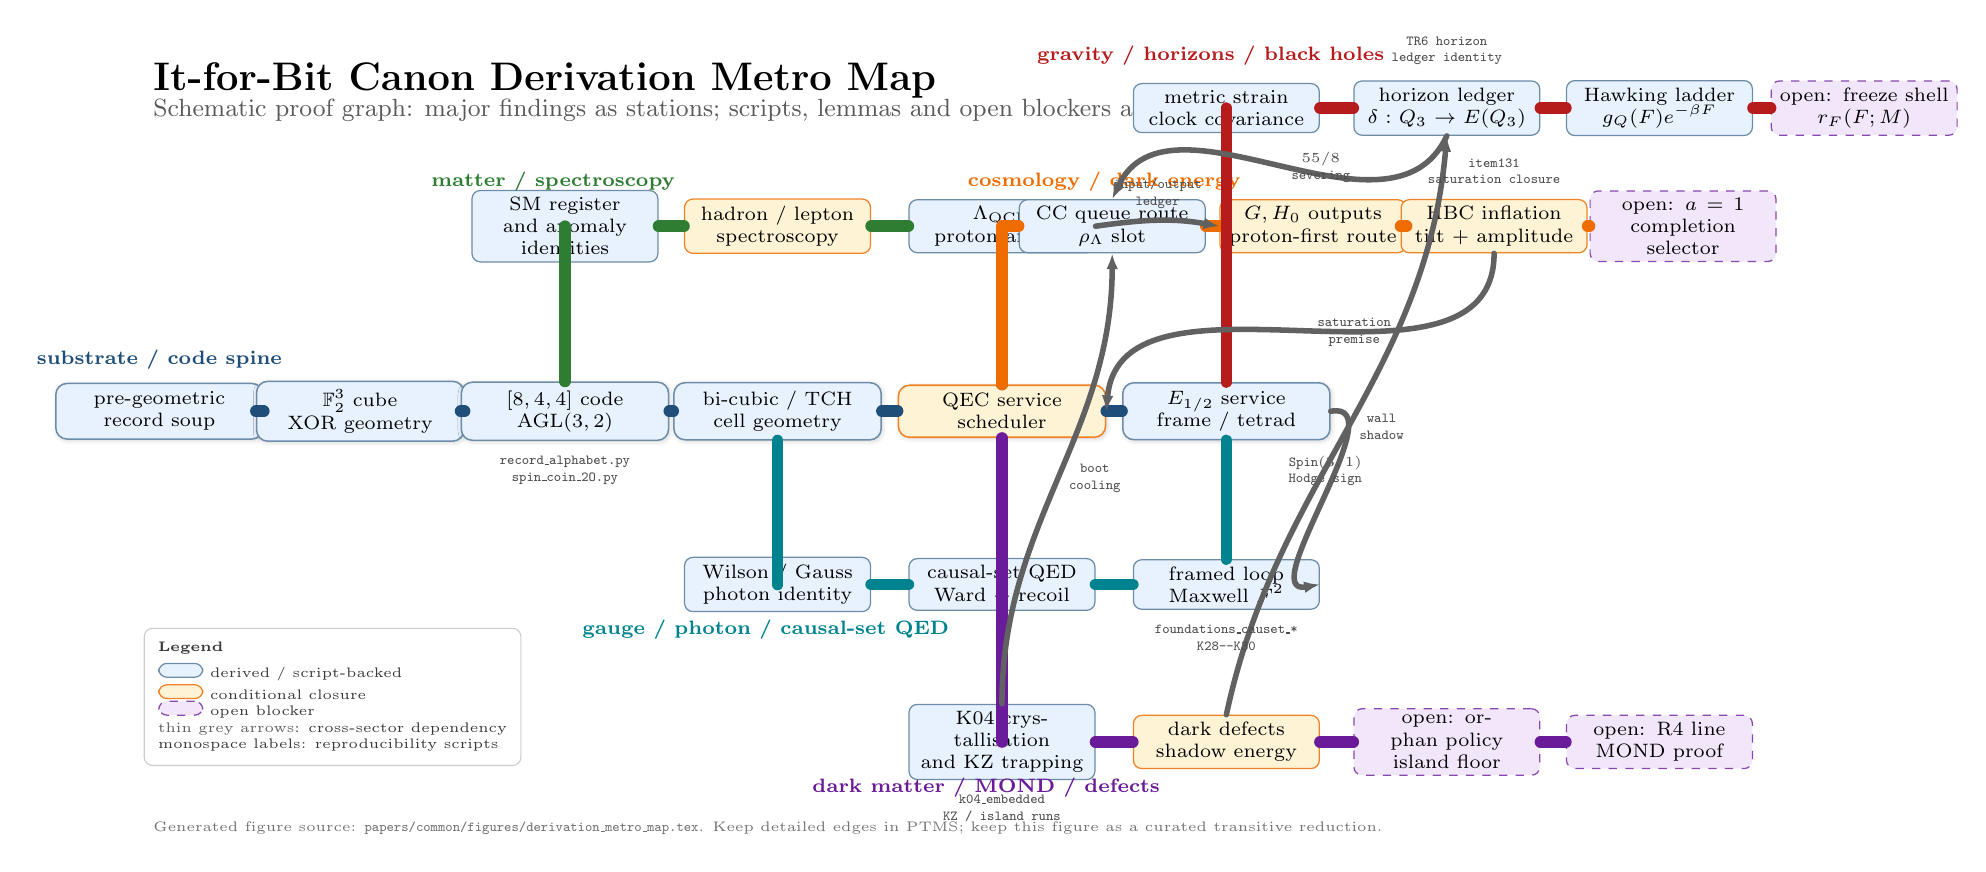
\begin{tikzpicture}[x=1cm,y=1cm]

% --- Title ---
\node[font=\Large\bfseries, anchor=west] at (-0.2,8.4)
  {It-for-Bit Canon Derivation Metro Map};
\node[font=\small, text=black!65, anchor=west] at (-0.2,8.02)
  {Schematic proof graph: major findings as stations; scripts, lemmas and open blockers as edge labels.};

% --- Foundation spine coordinates ---
\node[transfer, derived] (soup) at (0,4.2) {pre-geometric\\record soup};
\node[transfer, derived] (cube) at (2.55,4.2) {$\mathbb F_2^3$ cube\\XOR geometry};
\node[transfer, derived] (code) at (5.15,4.2) {$[8,4,4]$ code\\AGL$(3,2)$};
\node[transfer, derived] (cell) at (7.85,4.2) {bi-cubic / TCH\\cell geometry};
\node[transfer, conditional] (service) at (10.7,4.2) {QEC service\\scheduler};
\node[transfer, derived] (frame) at (13.55,4.2) {$E_{1/2}$ service\\frame / tetrad};

% Foundation route.
\draw[route, substrate] (soup) -- (cube) -- (code) -- (cell) -- (service) -- (frame);
\node[labelbox, text=substrate] at (0.0,4.85) {substrate / code spine};

% --- Matter line ---
\node[station, derived] (fermions) at (5.15,6.55) {SM register\\and anomaly identities};
\node[station, conditional] (spectra) at (7.85,6.55) {hadron / lepton\\spectroscopy};
\node[station, derived] (proton) at (10.7,6.55) {$\Lambda_{\rm QCD}$\\proton anchor};
\draw[route, matter] (code.north) |- (fermions) -- (spectra) -- (proton) |- (service.north);
\node[labelbox, text=matter] at (5.0,7.12) {matter / spectroscopy};

% --- Gauge and QED line ---
\node[station, derived] (wilson) at (7.85,2.0) {Wilson / Gauss\\photon identity};
\node[station, derived] (ward) at (10.7,2.0) {causal-set QED\\Ward + recoil};
\node[station, derived] (maxwell) at (13.55,2.0) {framed loop\\Maxwell $F^2$};
\draw[route, gauge] (cell.south) |- (wilson) -- (ward) -- (maxwell) |- (frame.south);
\node[labelbox, text=gauge] at (7.7,1.42) {gauge / photon / causal-set QED};

% --- Cosmology line ---
\node[station, derived] (cc) at (12.1,6.55) {CC queue route\\$\rho_\Lambda$ slot};
\node[station, conditional] (h0g) at (14.65,6.55) {$G,H_0$ outputs\\proton-first route};
\node[station, conditional] (hbc) at (16.95,6.55) {HBC inflation\\tilt + amplitude};
\node[station, open] (epoch) at (19.35,6.55) {open: $a=1$\\completion selector};
\draw[route, cosmo] (service.north) |- (cc) -- (h0g) -- (hbc) -- (epoch);
\node[labelbox, text=cosmo] at (12.0,7.12) {cosmology / dark energy};

% --- Dark sector / defect line ---
\node[station, derived] (k04) at (10.7,0.0) {K04 crystallisation\\and KZ trapping};
\node[station, conditional] (debris) at (13.55,0.0) {dark defects\\shadow energy};
\node[station, open] (orphan) at (16.35,0.0) {open: orphan policy\\island floor};
\node[station, open] (mond) at (19.05,0.0) {open: R4 line\\MOND proof};
\draw[route, dark] (service.south) |- (k04) -- (debris) -- (orphan) -- (mond);
\node[labelbox, text=dark] at (10.5,-0.58) {dark matter / MOND / defects};

% --- Gravity and black-hole line ---
\node[station, derived] (metric) at (13.55,8.05) {metric strain\\clock covariance};
\node[station, derived] (delta) at (16.35,8.05) {horizon ledger\\$\delta:Q_3\to E(Q_3)$};
\node[station, derived] (hawking) at (19.05,8.05) {Hawking ladder\\$g_Q(F)e^{-\beta F}$};
\node[station, open] (freeze) at (21.65,8.05) {open: freeze shell\\$r_F(F;M)$};
\draw[route, gravity] (frame.north) |- (metric) -- (delta) -- (hawking) -- (freeze);
\node[labelbox, text=gravity] at (13.35,8.72) {gravity / horizons / black holes};

% --- Cross-sector transfer edges ---
\draw[thinroute, method, -{Latex[length=2mm]}] (proton.east) to[out=8,in=170] node[proof, above] {input/output\\ledger} (h0g.west);
\draw[thinroute, method, -{Latex[length=2mm]}] (delta.south) to[out=-115,in=65] node[proof, right] {$55/8$\\severing} (cc.north);
\draw[thinroute, method, -{Latex[length=2mm]}] (frame.east) to[out=10,in=190] node[proof, above] {Spin$(3,1)$\\Hodge sign} (maxwell.east);
\draw[thinroute, method, -{Latex[length=2mm]}] (k04.north) to[out=90,in=-90] node[proof, right] {boot\\cooling} (cc.south);
\draw[thinroute, method, -{Latex[length=2mm]}] (debris.north) to[out=78,in=-95] node[proof, right] {wall\\shadow} (delta.south);
\draw[thinroute, method, -{Latex[length=2mm]}] (hbc.south) to[out=-90,in=85] node[proof, right] {saturation\\premise} (service.east);

% --- Script labels ---
\node[proof, below=2pt of code] {record\_alphabet.py\\spin\_coin\_2O.py};
\node[proof, below=2pt of maxwell] {foundations\_causet\_*\\K28--K30};
\node[proof, above=2pt of delta] {TR6 horizon\\ledger identity};
\node[proof, below=2pt of k04] {k04\_embedded\\KZ / island runs};
\node[proof, above=2pt of hbc] {item131\\saturation closure};

% --- Legend ---
\node[legend, draw=black!20, rounded corners=3pt, fill=white, anchor=north west, inner sep=5pt] at (-0.2,1.45) {
  \textbf{Legend}\\[2pt]
  \tikz{\node[station, derived, minimum width=0.5cm, text width=0.35cm]{};} derived / script-backed\\
  \tikz{\node[station, conditional, minimum width=0.5cm, text width=0.35cm]{};} conditional closure\\
  \tikz{\node[station, open, minimum width=0.5cm, text width=0.35cm]{};} open blocker\\
  \textcolor{method}{thin grey arrows}: cross-sector dependency\\
  monospace labels: reproducibility scripts
};

% --- Status footer ---
\node[font=\tiny, text=black!55, anchor=west] at (-0.2,-1.1)
  {Generated figure source: \texttt{papers/common/figures/derivation\_metro\_map.tex}. Keep detailed edges in PTMS; keep this figure as a curated transitive reduction.};

\end{tikzpicture}
\end{document}
